\documentclass{report}
\usepackage[T1]{fontenc} % Fontes T1
\usepackage[utf8]{inputenc} % Input UTF8
%\usepackage[backend=biber, style=ieee]{biblatex} % para usar bibliografia
%\usepackage{csquotes}
\usepackage[portuguese]{babel}
%\usepackage[portuguese]{babel} %Usar língua portuguesa
\usepackage{blindtext} % Gerar texto automaticamente
\usepackage[printonlyused]{acronym}
\usepackage{hyperref} % para autoref
%\usepackage{graphicx}
\usepackage[pdftex]{color,graphicx}

\usepackage{amsmath}

% Pacote para a definição de novas cores
\usepackage{xcolor}
% Definindo novas cores
\definecolor{verde}{rgb}{0.25,0.5,0.35}
\definecolor{jpurple}{rgb}{0.5,0,0.35}
\definecolor{darkgreen}{rgb}{0.0, 0.2, 0.13}
%\definecolor{oldmauve}{rgb}{0.4, 0.19, 0.28}
% Configurando layout para mostrar codigos Java
\usepackage{listings}

\newcommand{\estiloC}{
\lstset{
    language=C++,
    basicstyle=\ttfamily\small,
    keywordstyle=\color{jpurple}\bfseries,
    stringstyle=\color{red},
    commentstyle=\color{verde},
    morecomment=[s][\color{blue}]{/**}{*/},
    extendedchars=true,
    showspaces=false,
    showstringspaces=false,
    numbers=left,
    numberstyle=\tiny,
    breaklines=true,
    backgroundcolor=\color{cyan!10},
    breakautoindent=true,
    captionpos=b,
    xleftmargin=0pt,
    tabsize=2
}}


\bibliography{bibliografia}


\begin{document}
%%
% Definições
%
\def\titulo{Informação e Codificação}
\def\subtitle{Projeto 1}
\def\data{30 de outubro de 2022}
\def\autores{Bruno Silva (97931)brunosilva16@ua.pt \\ Marta Oliveira (97613) marta.alex@ua.pt \\ Mariana Silva (98392) marianabarbara@ua.pt}
\def\versao{VERSAO 1}
\def\departamento{DETI}
\def\empresa{Universidade de Aveiro}
\def\logotipo{ua.pdf}
%
%%%%%% CAPA %%%%%%
%
\renewcommand{\contentsname}{Índice}
\begin{titlepage}

\begin{center}
%
\vspace*{15mm}
%
{\Huge \titulo}\\
%
\vspace{10mm}
%
{\Huge \subtitle}\\
%
\vspace{10mm}
%
{\Large \empresa}\\
%
\vspace{10mm}
%
{\LARGE \autores}\\ 
%
\vspace{10mm}
%
\begin{figure}[h]
\center
\includegraphics{\logotipo}
\end{figure}
%
\vspace{30mm}
\end{center}
%
\begin{flushright}
\versao
\end{flushright}
\end{titlepage}

%%  Página de Título %%
\title{%
{\Huge\textbf{\titulo}}\\
{\Large \departamento\\ \empresa}
}
%
\author{%
    \autores
}
%
\date{\data}
%
\maketitle

\pagenumbering{roman}



%%%%%% Agradecimentos %%%%%%
% Segundo glisc deveria aparecer após conclusão...
%\renewcommand{\abstractname}{Agradecimentos}
%\begin{abstract}
%Eventuais agradecimentos.
%Comentar bloco caso não existam agradecimentos a fazer.
%\end{abstract}


\tableofcontents
 %\listoftables     % descomentar se necessário
 \listoffigures    % descomentar se necessário


%%%%%%%%%%%%%%%%%%%%%%%%%%%%%%%
\clearpage
\pagenumbering{arabic}

%%%%%%%%%%%%%%%%%%%%%%%%%%%%%%%%
\chapter{Introdução}
\label{chap.introducao}
\paragraph{}
O presente relatório tem como objetivo descrever a resolução do Projeto 1 desenvolvido no âmbito da unidade curricular de Informação e Codificação.

\paragraph{}
O código desenvolvido para o projeto encontra-se disponível em \url{https://github.com/brunosilva16/IC}

\paragraph{}
Para este projeto utilizamos a libraria \textit{libsndfile} e o programa \textit{gnuplot}. 
No ficheiro README.md no repositório estão as indicações de como compilar cada exercício.


\chapter{Parte I}
\label{chap.ParteI}
\section{Exercício 2}
\paragraph{}
Neste exercício era pedido para providenciar um histograma da média dos canais (mid channel) e a diferença de canais (side channel) quando o áudio é estéreo, isto é, com dois canais.
\begin{center}
    MID CHANNEL= (L + R)/2\\
    SIDE CHANNEL = (L - R)/2
\end{center}

Para isso, criámos um programa que tem como argumentos de entrada um ficheiro de som (tipo wav) existente.
Com o uso da biblioteca libsndfile conseguimos guardar a informação de cada canal num vetor.
Para proceder à contagem de cada ocorrência de valores, recorremos a uma estrutura de dados do tipo vetor que por sua vez usa um map em que as chaves (tipo short)são os valores lido do ficheiro de áudio e estão associadas ao número de ocorrências.
\paragraph{}
Finalmente, para apresentarmos a informação num histograma recorremos ao gnuplot.
\paragraph{}
De seguida, mostramos os comandos necessários para verificar os resultados.\\

\textcolor{red}{Como compilar o exercício 2:}
\textbf{make wav\textunderscore hist}

\textcolor{red}{Comando para executar o programa:} \textbf{../sndfile-example-bin/wav\textunderscore hist <input file> <channel>}
\paragraph{}
O channel pode ser 0 or 1 para canal esquerdo ou direito respetivamente, s para side e m for mid.\\
\textcolor{red}{Para abrir os histogramas:}\\
\textbf{gnuplot}\\
\textbf{plot "histM.dat"}\\
\textbf{plot "histS.dat"}\\
\textbf{plot "hist.dat"}\\
No eixo das abcissas estão representados todos os valores das samples e no eixo das coordenadas está representado o número de ocorrências
\begin{figure} [h!]
\center
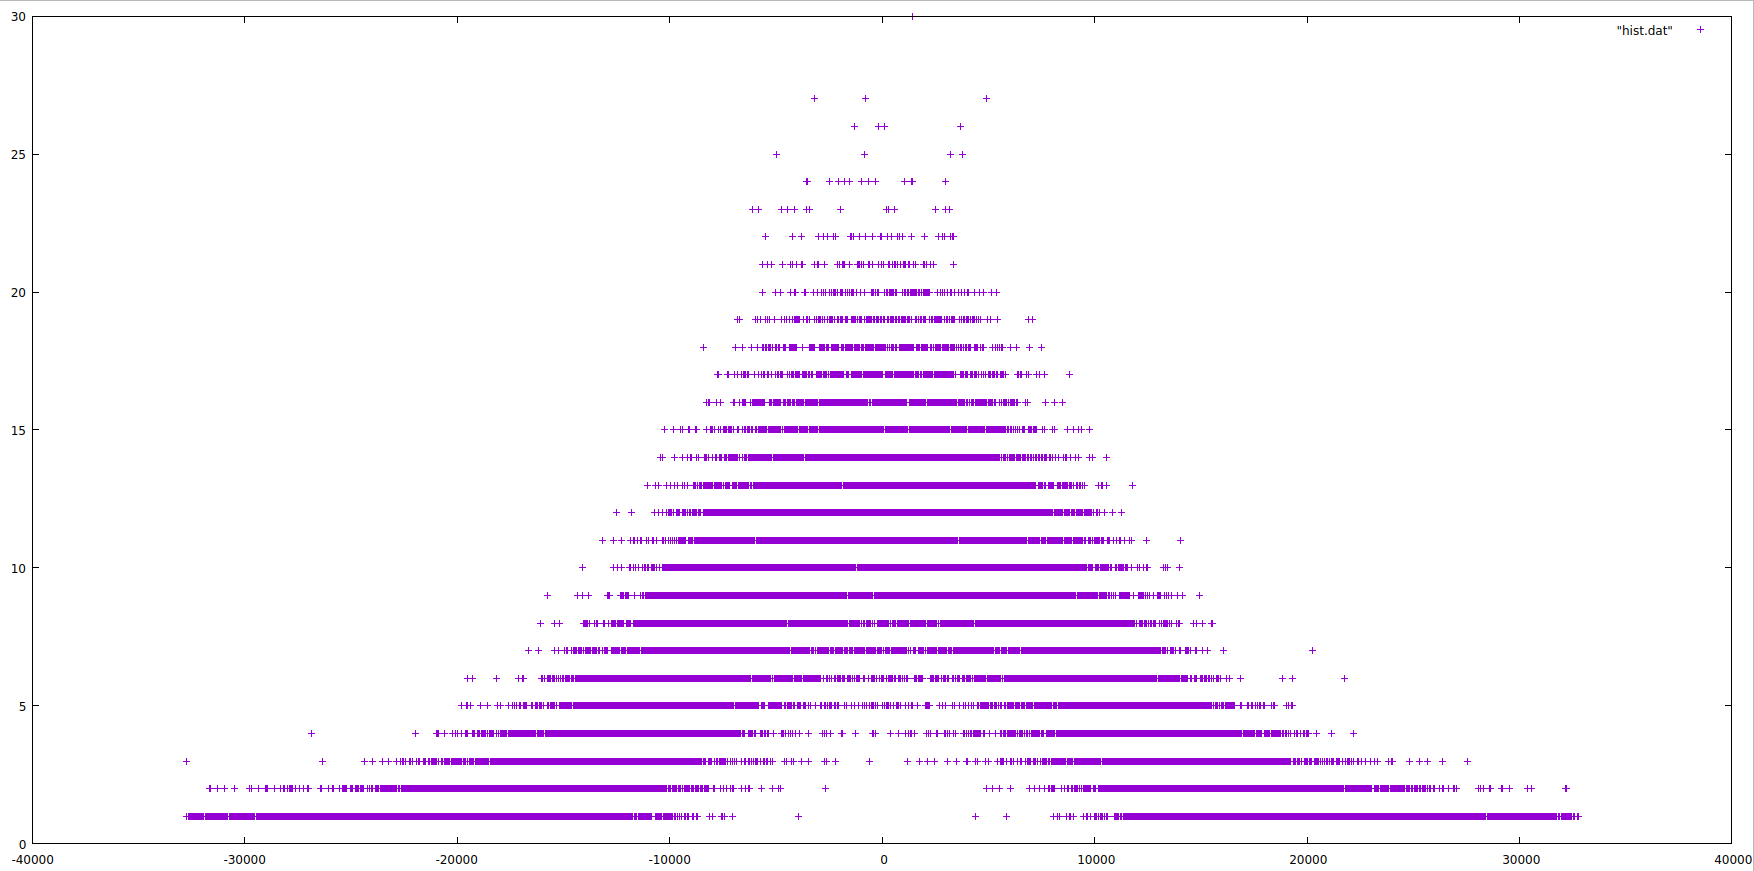
\includegraphics[height=6cm]{hist.png}
\caption{hist.dat}
\label{fig: hist.dat}
\end{figure}

\begin{figure} [h!]
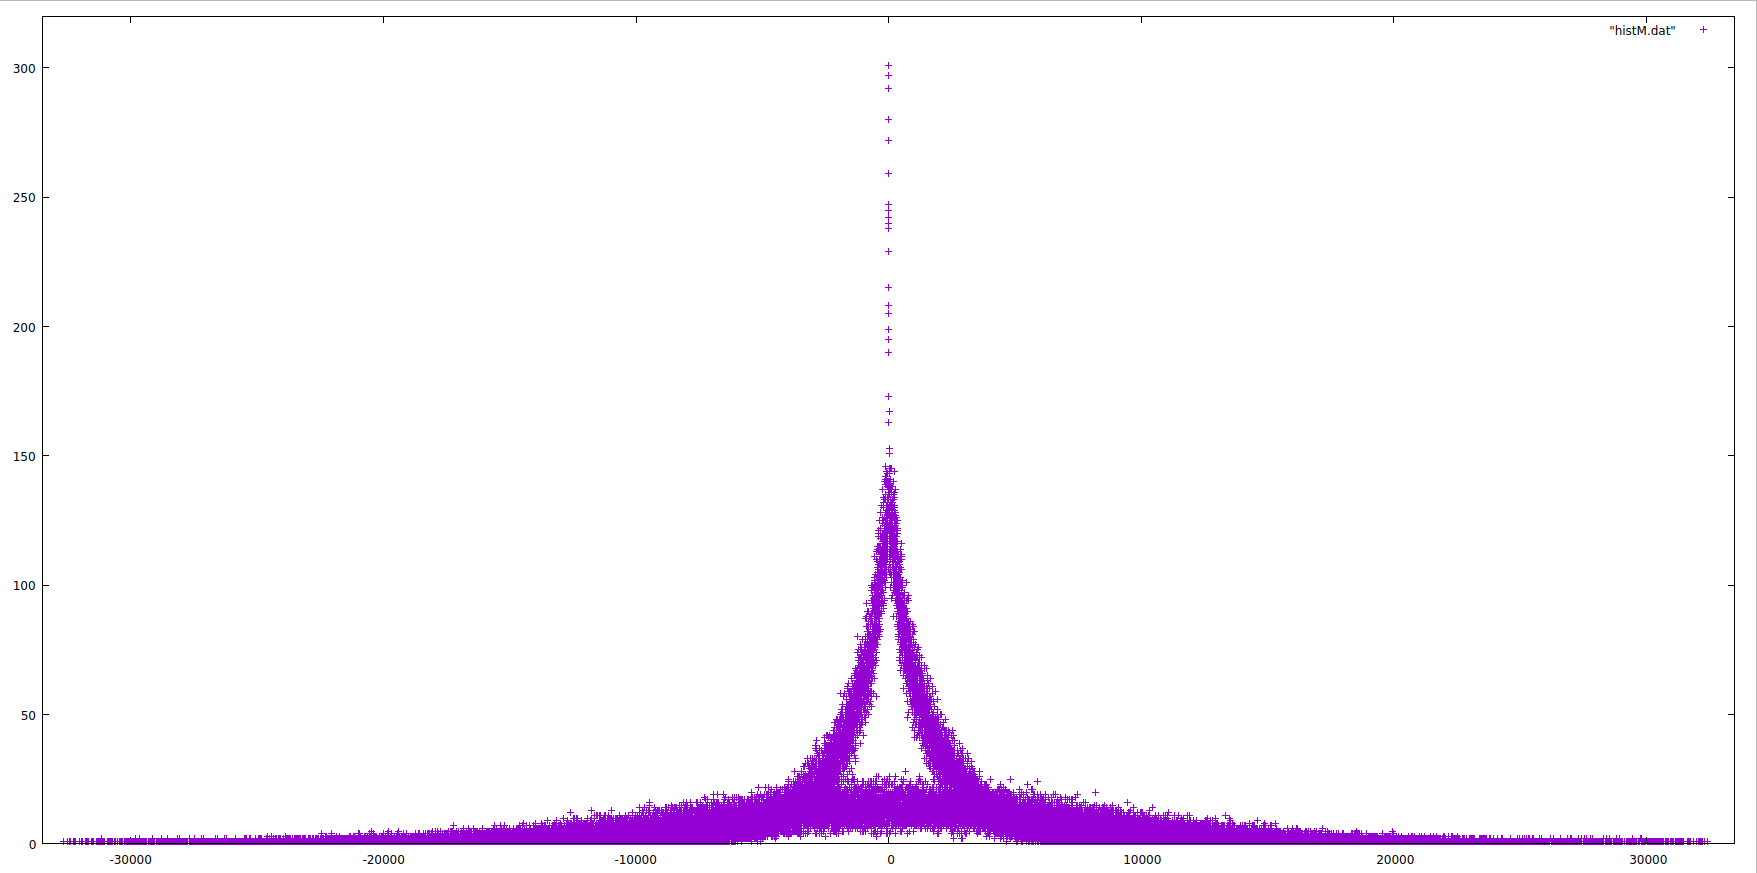
\includegraphics[height=6cm]{histM.png}
\caption{histM.dat}
\label{fig: histM.dat}
\end{figure}
\paragraph{}
\begin{center}
\begin{figure} [h!]
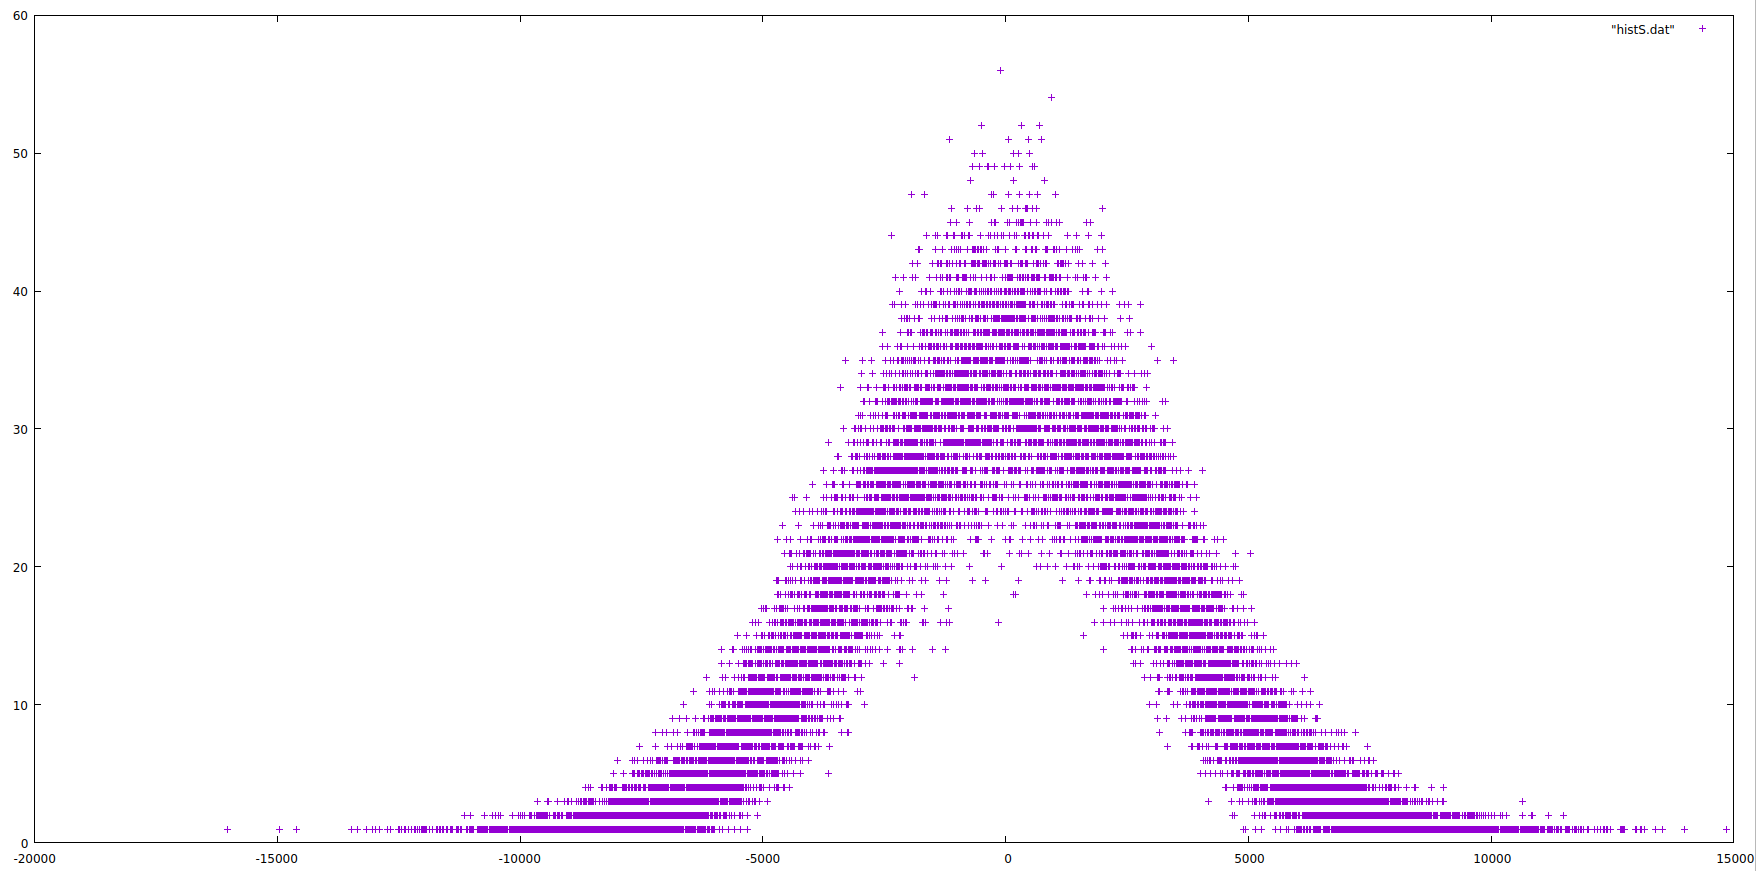
\includegraphics[height=6cm]{histS.png}
\caption{histS.dat}
\label{fig: histS.dat}
\end{figure}
\end{center}
.


\newpage
\section{Exercício 3}
\paragraph{}
O objetivo deste exercício era a quantização de som, isto é, reduzir o número de bits usados para representar cada sample de um ficheiro de aúdio.
\paragraph{}
O processo de quantização de som representa a transformação de um sinal contínuo num sinal discreto. Esta técnica é irreversível, uma vez que implica perdas de informação.
\paragraph{}
Para este exercício, o utilizador irá inserir o ficheiro que quer quantizar, o nome do ficheiro onde irá ser guardado o resultado e o número de bits a descartar. Este valor tem de estar entre 1 a 16 bits pois os ficheiro WAV fornecidos são compostos por amostras de 16 bits.\paragraph{}
Depois disso realizámos um deslocamento para a direita dos bits menos significativos da sample e, para não alterar o tamanho dela, recolocamos os bits a 0 realizando um descolamento para a esquerda. Desta forma, foi reduzida/eliminada a informação menos significativa da sample. 

\begin{scriptsize}
\estiloC
\begin{lstlisting}[caption={Código fonte em C}, label=lst:javacode]
	void quant_samples(const std::vector<short>& samples, size_t bits_disc) {
    for(auto sample : samples){
      sample = (sample >> bits_disc) << bits_disc;
      samples_quant.push_back(sample);
		}
	}
\end{lstlisting}
\end{scriptsize}
\\
\paragraph{}
O ficheiro produzido apresenta mais ou menos ruído dependendo do números de bits a descartar.\\
\textcolor{red}{Como compilar o exercício 3:}
\textbf{make wav\textunderscore quant}\\
\textcolor{red}{Comando para executar o programa:}
\textbf{../sndfile-example-bin/wav\textunderscore quant <input filename> <output filename> <number of bits to discard>}

\section{Exercício 4}
\paragraph{}
Uma vez que a operação de quantização introduz erros, é importante calcular a quantidade de ruído que introduzimos.
%colocar aqui as expressoes entao que usamos%
\paragraph{} 
\begin{equation}
SNR = 10 \log_{10} \frac{E_x}{E_r}  dB
\end{equation}
\paragraph{}

Onde Ex é a energia do sinal e tem a seguinta fórmula: 
\begin{equation}
sum_ {N}|x(n)^2| 
\end{equation}
\paragraph{}
M(n) é o sinal do ruído e tem de equação: 
\begin{equation}
x(n)-\overset{-}{x}(n)
\end{equation}
 \paragraph{} 
Onde x(n) são samples do áudio original e \overset{-}{x}(n) \text{ são as samples de áudio comprimido}. \paragraph{}

Er\text{ é a energia do sinal do ruído}:  
\begin{equation}
sum_{N}|(M(n)^2|
\end{equation}

\paragraph{}
É de observar que pelo quanto mais comprimido for o som menor será o valor de SNR.
\paragraph{}
Assim, para correr o programa o utilizador precisa de fornecer um ficheiro de áudio e de seguida o ficheiro de aúdio comprimido correspondente. Se isso se verificar, os cálculos com as fórmulas anteriores vão ser realizados.
\begin{scriptsize}
\estiloC
\begin{lstlisting}[caption={Código fonte em C}, label=lst:javacode]
	size_t nFrames;
    double signal_energy = 0, noise_energy = 0;
    double SNR;
    double maxError = 0, tmpError;

    while((nFrames = sndFileO.readf(samples_original.data(), FRAMES_BUFFER_SIZE))) {
        sndFileQ.readf(samples_quant.data(), FRAMES_BUFFER_SIZE);

        samples_original.resize(nFrames * sndFileO.channels());
        samples_quant.resize(nFrames * sndFileQ.channels());

        for (long int i = 0; i < (int)samples_original.size(); i++) {
            signal_energy += pow(samples_original[i], 2);
            tmpError = abs(samples_original[i] - samples_quant[i]);
            noise_energy += pow(tmpError, 2);
            
            if(tmpError > maxError){
                maxError = tmpError;
            }
        }    
    }

    SNR = 10 * log10(signal_energy / noise_energy);
    cout << "SNR: " << SNR << " dB\nMaximum per sample absolute error: " << maxError << endl;
\end{lstlisting}
\end{scriptsize}
\textcolor{red}{Como compilar o exercício 4:}
\textbf{make wav\textunderscore cmp}\\
\textcolor{red}{Comando para executar o programa:}
\textbf{../sndfile-example-bin/wav\textunderscore cmp <original file> <quantized file>}

\section{Exercício 5}
\paragraph{}
No exercício 5, foi nos pedido para produzir efeitos em ficheiros de aúdio.
Começamos por produzir o eco. Para haver este efeito, temos que pegar em cada sample do som e adicionar uma sample (com k de atraso) que é multiplicada por um  ganho ('quantidade' de efeito) que o utilizador pretende efetuar:\\
\begin{center}
    y(n) = (x(n) + alpha * x(n-k))/(1+alpha)
\end{center}
\paragraph{}
Semelhante a este processo, temos o eco múltiplo, para isso já é necessário o programa ir buscar o resultado do eco anterior(função de realimentação) e voltar a processar dando o efeito de eco contínuo.
\begin{center}
    y(n) = (x(n) + alpha* \textbf{(y-delay)})/(1+alpha)    
\end{center}
 \paragraph{}
 Observámos que, no single\textunderscore eco, como o momento em que isso acontece é único ao longo do áudio torna-se díficil de o efeito ser perceptível.
\paragraph{}
Além disso, adicionámos o efeito invertido. Para isso, através do ciclo \textit{for}  trocou-se a ordem das samples.
 
\begin{scriptsize}
\estiloC
\begin{lstlisting}[caption={Código fonte em C}, label=lst:javacode] 
 else if(wanted_effect == "reverse") {
        while((nFrames = sfhIn.readf(samples.data(), FRAMES_BUFFER_SIZE))) {
            samples.resize(nFrames * sfhIn.channels());

            for (int i = (int)samples.size() - 1; i >= 0; i--) samples_out.insert(samples_out.end(), samples.at(i));
        }        
    }
\end{lstlisting}
\end{scriptsize} 
 \paragraph{}
 Por último, realizámos uma modulação do som. O som tem duas componentes importantes, a amplitude e a frequência. No caso de uma onda sonora, a amplitude representa um som com uma intensidade mais "alta" ou "baixa".
\paragraph{}
O fator de modulação vai ser a proporção de variação da amplitude da onda sonora. Como uma onda sonora tem metade do ciclo positivo e metade do ciclo negativo, a fórmula matemática para a modelação de som será:
 \begin{center}
    y(n) = x(n) * cos(2*pi*(f/fa)*n)  
 \end{center}
\\


\begin{scriptsize}
\estiloC
\begin{lstlisting}[caption={Código fonte em C}, label=lst:javacode] 
 else if(effect=="a"){
         while((size = sndFileIn.readf(samples_original.data(), FRAMES_BUFFER_SIZE))) {
            samples_original.resize(size * sndFileIn.channels());
            for (int i = 0; i < samples_original.size(); i++) {
                single_sample_out = samples_original.at(i) * cos((2 * M_PI * (0.1/fa) * i));
                samples_out.insert(samples_out.end(), single_sample_out);
            }
        }
    }
\end{lstlisting}
\end{scriptsize} 
\textcolor{red}{Como compilar o exercício 5:}
\textbf{make wav\textunderscore effects}\\
\textcolor{red}{Comando para executar o programa:}
\textbf{../sndfile-example-bin/wav\textunderscore effects <input file> <output\textunderscore file> <effect>}
\newpage
<effect> é 's' para eco único (single eco), 'm' para eco múltiplo, 'r' para revertido e 'a' para modelação de amplitude. De seguida, mostramos como se executa o programa para cada efeito. 
\begin{center}
\begin{figure} [h!]
\center
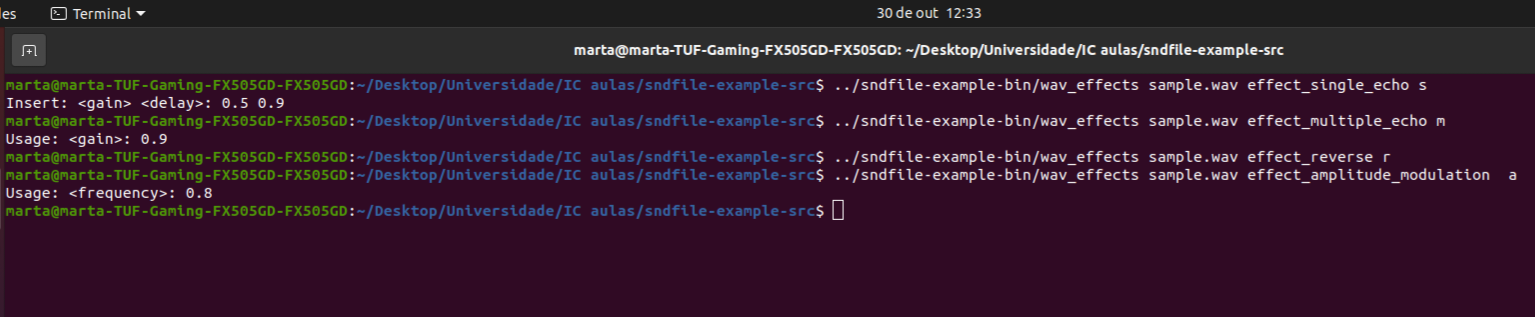
\includegraphics[width=15cm]{terminal.png}
\caption{terminal}
\label{fig: terminal}
\end{figure}
\end{center}
Na pasta do nosso projeto encontram-se os ficheiros produzidos nesta compilação.
\chapter{Parte II}
\label{chap.ParteII}
\section{Exercício 6}
\paragraph{}
A classe Bitstream que nos foi pedida permite a manipulação de um ficheiro bit a bit usando uma stream, sendo o \textit{char} o tipo primitivo mais pequeno possível de representar, ocupando apenas 1 byte de memória.
\paragraph{}
Para resolvermos como fazer as ações de manipulação de ficheiros criamos uma classe \textit{BitStream}.
A assinatura desta classe é demonstrada de seguida:
\begin{scriptsize}
\estiloC
\begin{lstlisting}[caption={Código fonte em C}, label=lst:javacode] 
class BitStream {
    private:
        fstream file;
        string filename;
        int mode; 
        int fileSize;  
        std::vector<int> buffer; // stores the bits of the current byte
        int currentPos; // stores the current bit position of reading/writting

    public:
        BitStream();
        BitStream(string filename, char mode);
        int readBit();
        std::vector<int> readNbits(int n);
        void writeBit(int bit);
        void writeNbits(std::vector<int>);
        std::vector<int> byteToBuffer(char c);
        char bufferToByte(std::vector<int>);
        int getFileSize();
        void close();
};
\end{lstlisting}
\end{scriptsize} 
\paragraph{}
Como os nomes indicam, temos funções para ler e escrever bit e N bits.
\paragraph{}
O que se tem de ter em conta na manipulação de ficheiros é que não se pode escrever um único bit diretamente num ficheiro. A unidade de I/0 de leitura/escrita é um byte (8-bits). 
Por isso, tem de se guardar tudo em blocos de 8 bits e depois escrever.

\begin{scriptsize}
\estiloC
\begin{lstlisting}[caption={Código fonte em C}, label=lst:javacode] 
void BitStream::writeBit(int bit)
{
    if(mode == 1) {
        cerr <<"Cannot write bit in read mode"<< endl;
        exit(1);
    }
    // if the current bit position is 8, the byte will be written and the current position will be set to 0
    if (currentPos == 8){
        char byte = bufferToByte(buffer);
        file.write(&byte, 1);
        currentPos = 0;
    }
    // if the current pos is 0, the buffer needs to be initialized
    if (currentPos == 0) buffer = std::vector<int>(8);

    buffer[currentPos] = bit; // put the current bit on the buffer
    currentPos++;
}
};
\end{lstlisting}
\end{scriptsize} 
Para a leitura cada caráter que é lido(bit a 0 ou a 1) do ficheiro de entrada será interpretado como um bit do buffer que será utilizado futuramente para a escrita do ficheiro binário.
\begin{scriptsize}
\estiloC
\begin{lstlisting}[caption={Código fonte em C}, label=lst:javacode] 
int BitStream::readBit() {
    if (mode ==0) {
        cerr << "Cannot read file in write mode" << endl;
        exit(1);
    }
    
    if (currentPos == 0) {
        char byte;
        file.read(&byte, 1);
        buffer = byteToBuffer(byte);
    }
    int bit = buffer[currentPos];
    currentPos = (currentPos + 1) % 8;
    return bit;
}
\end{lstlisting}
\end{scriptsize} 



\section{Exercício 7}
\paragraph{}
De forma a testa a nossa classe criámos dois programas:\textit{encoder} e \textit{decoder}.
\paragraph{}
O encoder pega num ficheiro de texto que contém 0's e 1´s em que cada conjunto de 8 bits é formado num byte.
\paragraph{}
Como os valores binários são representados em ASCII e sabendo que '0' em ASCII é 48 e '1' é 49 nós iremos escrever no vetor o valor real lido do ficheiro. Por exemplo, se o valor lido do ficheiro for 1 fica 49-48 que é 1.
\begin{scriptsize}
\estiloC
\begin{lstlisting}[caption={Código fonte em C}, label=lst:javacode] 
 // read data as a block:
    inputFile.read (buffer,length);
    cout << "Length of the input file: " << length << endl;
    cout << "Content of the input file: '" << buffer << "'"<< endl;

    BitStream BSout (outputFileName, 'w') ;

    //write the bits to the output file
    vector<int> bits;
    for (int i = 0; i < length; i++){
        bits.push_back(buffer[i] - '0');  // 
    }
    BSout.writeNbits(bits);
    BSout.close();
\end{lstlisting}
\end{scriptsize}
\paragraph{}
Para compilar este encoder basta:\\
\textcolor{red}{Compilar o encoder:}
\textbf{make encoder}\\
\textcolor{red}{Comando para executar o programa:}
\textbf{../sndfile-example-bin/encoder  <input filename> <output filename>}
\paragraph{} Para ver os resultados, basta abrir o output(ficheiro .bin) que foi escrito no terminal.
\paragraph{}
O decoder faz a transformação oposta.
\begin{scriptsize}
\estiloC
\begin{lstlisting}[caption={Código fonte em C}, label=lst:javacode] 
 //read the bits from the input file
    vector<int> bits;
    bits = BSin.readNbits(BSin.getFileSize() * 8);
    BSin.close();

    //write the bits to the output file
    for (int i = 0; i < bits.size(); i++){
        outputFile << bits[i];
    }
    outputFile.close();

    return 0;
\end{lstlisting}
\end{scriptsize} 
\textcolor{red}{Como compilar o decoder:}
\textbf{make decoder}\\
\textcolor{red}{Comando para executar o programa:}
\textbf{../sndfile-example-bin/decoder <input filename> <output filename>}



\chapter*{Contribuições dos autores}
\paragraph{}
O trabalho foi dividido entre os três, sendo as percentagens para cada um as seguintes:
\paragraph{}
Bruno Silva -> 35\%
\paragraph{}
Marta Oliveira -> 35\%
\paragraph{}
Mariana Silva -> 30\%

\chapter*{Webgrafia}
\paragraph{}
\url{https://elearning.ua.pt/pluginfile.php/3743066/mod_resource/content/4/ic-notas.pdf}
\paragraph{}
\url{https://cplusplus.com/forum/beginner/94731/}
\paragraph{}
\url{https://www.dir.uniupo.it/pluginfile.php/154365/mod_resource/content/1/Lecture\%204_6\%20-\%20Quantization\%20and\%20reconstruction.pdf}
\paragraph{}
\url{https://www.sciencedirect.com/topics/engineering/uniform-quantization}
\paragraph{}
\url{https://www.willpirkle.com/forum/algorithm-design/bit-reduction/}
%%%%%%%%%%%%%%%%%%%%%%%%%%%%%%%%%

%\printbibliography

\end{document}
